\chapter{Architektura i struktura aplikacji}
\label{ch:architektura}

\section{Architektura aplikacji}
Aplikacja opiera się na architekturze trójwarstwowej, oddzielającej logikę biznesową od interfejsu i bazy danych. W projekcie zastosowano wzorzec architektoniczny MVVM\cite{MicrosoftMVVM} (Model-View-ViewModel), charakterystyczny dla technologii WPF. Umożliwia on łatwiejsze zarządzanie kodem i rozbudowywanie projektu.

Wzorzec MVVM dzieli aplikację na trzy niezależne komponenty:
\begin{itemize}
    \item \textbf{Model} -- przechowuje dane oraz reguły biznesowe aplikacji. Rolę modelu w projekcie pełnią klasy odpowiadające tabelom w bazie danych.
    \item \textbf{View} -- interfejs użytkownika zdefiniowany w języku XAML. Odpowiada za prezentację danych i interakcję z użytkownikiem, nie zawierając przy tym żadnej logiki biznesowej.
    \item \textbf{ViewModel} -- stanowi warstwę pośredniczącą między Modelem a Widokiem. Dostarcza dane z modelu w formie dostosowanej do bindowania w interfejsie użytkownika oraz obsługuje zdarzenia.
\end{itemize}

\section{Struktura folderów i organizacja kodu}
Kod źródłowy projektu \texttt{RockGym} został zorganizowany w przejrzystą strukturę katalogów, co ułatwia zarządzanie aplikacją i jej późniejszą rozbudowę. Główne foldery projektu to:
\begin{itemize}
    \item \textbf{Models} -- zawiera klasy definiujące struktury danych, takie jak \texttt{User.cs}, \texttt{Fingerprint.cs}, \texttt{Entrance.cs} czy \texttt{Offer.cs}. Stanowią one odzwierciedlenie schematu relacyjnej bazy danych.
    \item \textbf{Views} -- przechowuje pliki XAML wraz z ich plikami \textit{code-behind}. Znajdują się tu główne okna aplikacji (np. \texttt{MainWindow.xaml}, \texttt{LoginWindow.xaml}, \texttt{FingerprintScannerWindow.xaml}) oraz widoki poszczególnych modułów, m.in. sprzedaży (\texttt{TransactionsView.xaml}) i zarządzania klientami (\texttt{CustomersView.xaml}).
    \item \textbf{ViewModels} -- zbiór klas realizujących logikę biznesową dla poszczególnych widoków, m.in. \texttt{MainViewModel.cs}, \texttt{FingerprintScannerViewModel.cs} czy \texttt{LoginViewModel.cs}. Podfolder \texttt{Base} przechowuje klasy bazowe implementujące powiadamianie o zmianach właściwości (\texttt{INotifyPropertyChanged}).
    \item \textbf{Services} -- zawiera klasy usługowe, takie jak kontekst bazy danych (\texttt{RockGymContext.cs}), logika haszowania odcisków palców (\texttt{FingerprintHashing.cs}), konwertery widoków (\texttt{ByteToImageConverter.cs}) oraz mechanizmy powiadomień interfejsu (\texttt{CustomMessageBox.cs}).
\end{itemize}

\begin{figure}[H]
    \centering
    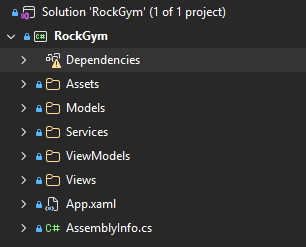
\includegraphics[width=0.6\linewidth]{figures/diagram_mvvm.png}
    \caption{Struktura folderów w projekcie.\label{fig:mvvm}}
\end{figure}

\section{Wzorce projektowe, walidacja i obsługa błędów}
Oprócz wzorca MVVM, w aplikacji zaimplementowano szereg mechanizmów zapewniających jej stabilność i niezawodność:
\begin{itemize}
    \item \textbf{Mechanizm powiązań danych (Data Binding)} -- widoki są w pełni zsynchronizowane z ViewModelami poprzez mechanizm bindowania, który wykorzystuje interfejs \texttt{INotifyPropertyChanged}. Akcje użytkownika, takie jak kliknięcia przycisków, realizowane są z użyciem wzorca \texttt{ICommand}.
    \item \textbf{Dostęp do bazy danych} -- realizowany jest przy użyciu technologii Object-Relational Mapping (ORM) i klasy \texttt{RockGymContext}. Upraszcza to zapytania do bazy MySQL i pozwala chronić aplikację przed atakami typu SQL injection.
    \item \textbf{Walidacja danych} -- przed wprowadzeniem danych do bazy (np. w oknach dodawania klientów czy edycji transakcji) aplikacja weryfikuje poprawność pól formularzy. Sprawdzane są wymogi dotyczące długości tekstów czy formatu danych.
    \item \textbf{Obsługa błędów i wyjątków} -- krytyczne operacje, takie jak łączenie z bazą danych czy wczytywanie plików obrazów odcisków palców, otoczone są blokami \texttt{try-catch}. W przypadku wystąpienia błędu (np. utraty połączenia z siecią, błędu skanowania), aplikacja zapobiega awarii i informuje o błędzie pracownika recepcji za pomocą dedykowanych okien dialogowych obsługiwanych przez klasę \texttt{CustomMessageBox}.
\end{itemize}
